\hspace{0.5 cm}
Pentru a putea interpreta datele rezultate le-am clasificat manual în tabel la fel ca și cele obținute folosind alpha-beta-CROWN. Câmpurile de tabel sunt identice cu cele de la alpha-beta-CROWN, singura excepție fiind ocurența a tipuri noi de rezultate, și anume:
\begin{itemize}
    \item \textbf{results (vnncomp2023/us)}: Poate avea valori sat/unsat/unknown/error; pentru \textbf{sat} și \textbf{unsat} interpretările sunt la fel ca și în cazul alpha-beta-CROWN, pentru \textbf{unknown} înseamnă că proprietatea nu a putut fi demonstrată, iar \textbf{error} rezultă atunci când a avut loc o eroare în timpul rulării tool-ului.
    Prima coloană cu rezultate reprezintă rezultatele obținute în competiție, iar a două coloană contine rezultatele obtinute de noi.
\end{itemize}

În tabelul \ref{fig:image2} se prezintă o analiză comparativă între rezultatele obținute în urma rulării proprii și cele obținute în cadrul competiției.

\begin{figure}[h]
\centering 
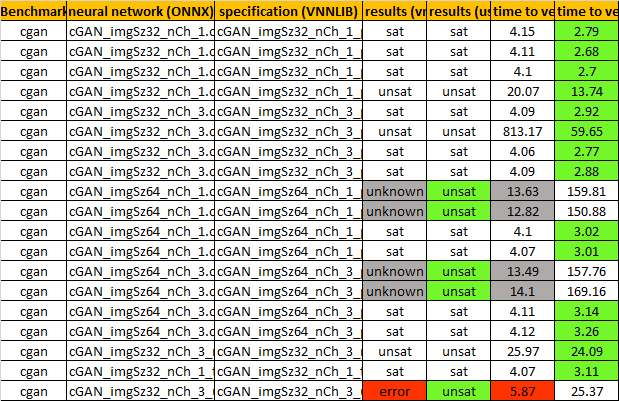
\includegraphics[width=0.8\linewidth]{imagini/interpretare rezultate/NeuralSAT_comp_vs_us.png}
\caption{Comparare rezultate NeuralSAT}
\label{fig:image2} 
\end{figure}
\

Comparând coloanele de \textit{results} am observat faptul că pentru toate instanțele am obținut valori satisfiabile sau nesatisfiabile. În schimb, competiția a obținut în cazul unor instanțe valori de \textit{unknown} si \textit{error}.

Graficul prezentat mai jos\ref{fig:image4}, evidențiază distribuirea timpilor de execuție pentru fiecare instanță în parte. În cadrul graficului de mai jos, se pot observa diferențele dintre timpii de execuție.
\begin{figure}[h]
\centering 
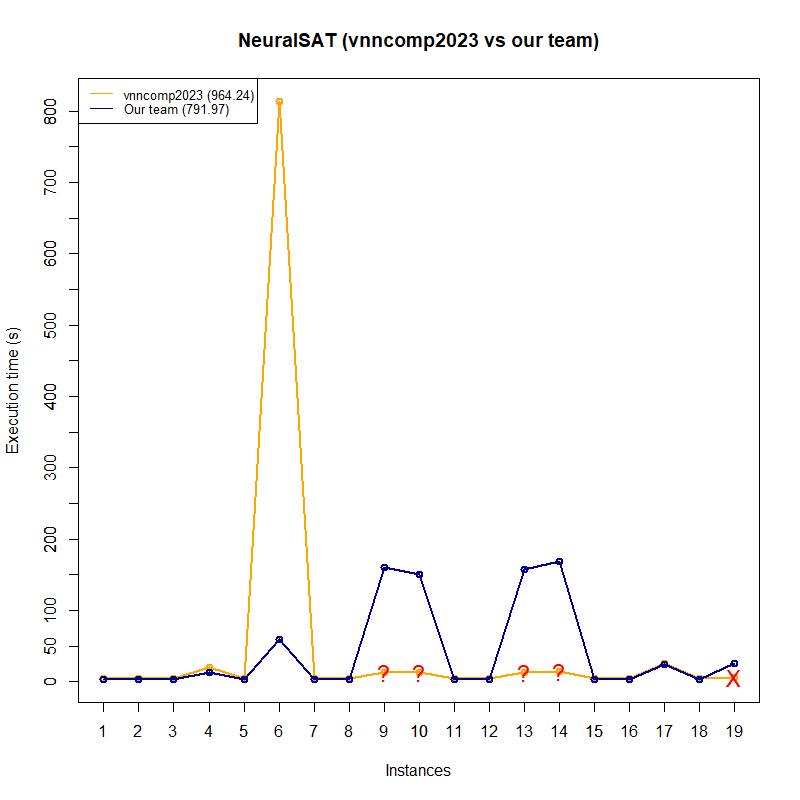
\includegraphics[width=0.8\linewidth]{imagini/interpretare rezultate/NeuralSAT_us_vs_vnncomp2023.png}
\caption{Comparare rezultate NeuralSAT}
\label{fig:image4} 
\end{figure}
\